\documentclass{standalone}
\usepackage{graphicx}
\usepackage{subfig}
\usepackage{tikz}
	\usetikzlibrary{spy}
\usepackage{siunitx}

\newcommand{\imsize}{\linewidth}
\newlength\imagewidth % needed for scalebars
\newlength\imagescale % ditto

\begin{document}%
%-------------
\begin{figure}
	\subfloat[Light microscopy image, \SI{10}{x} magnification.]{
		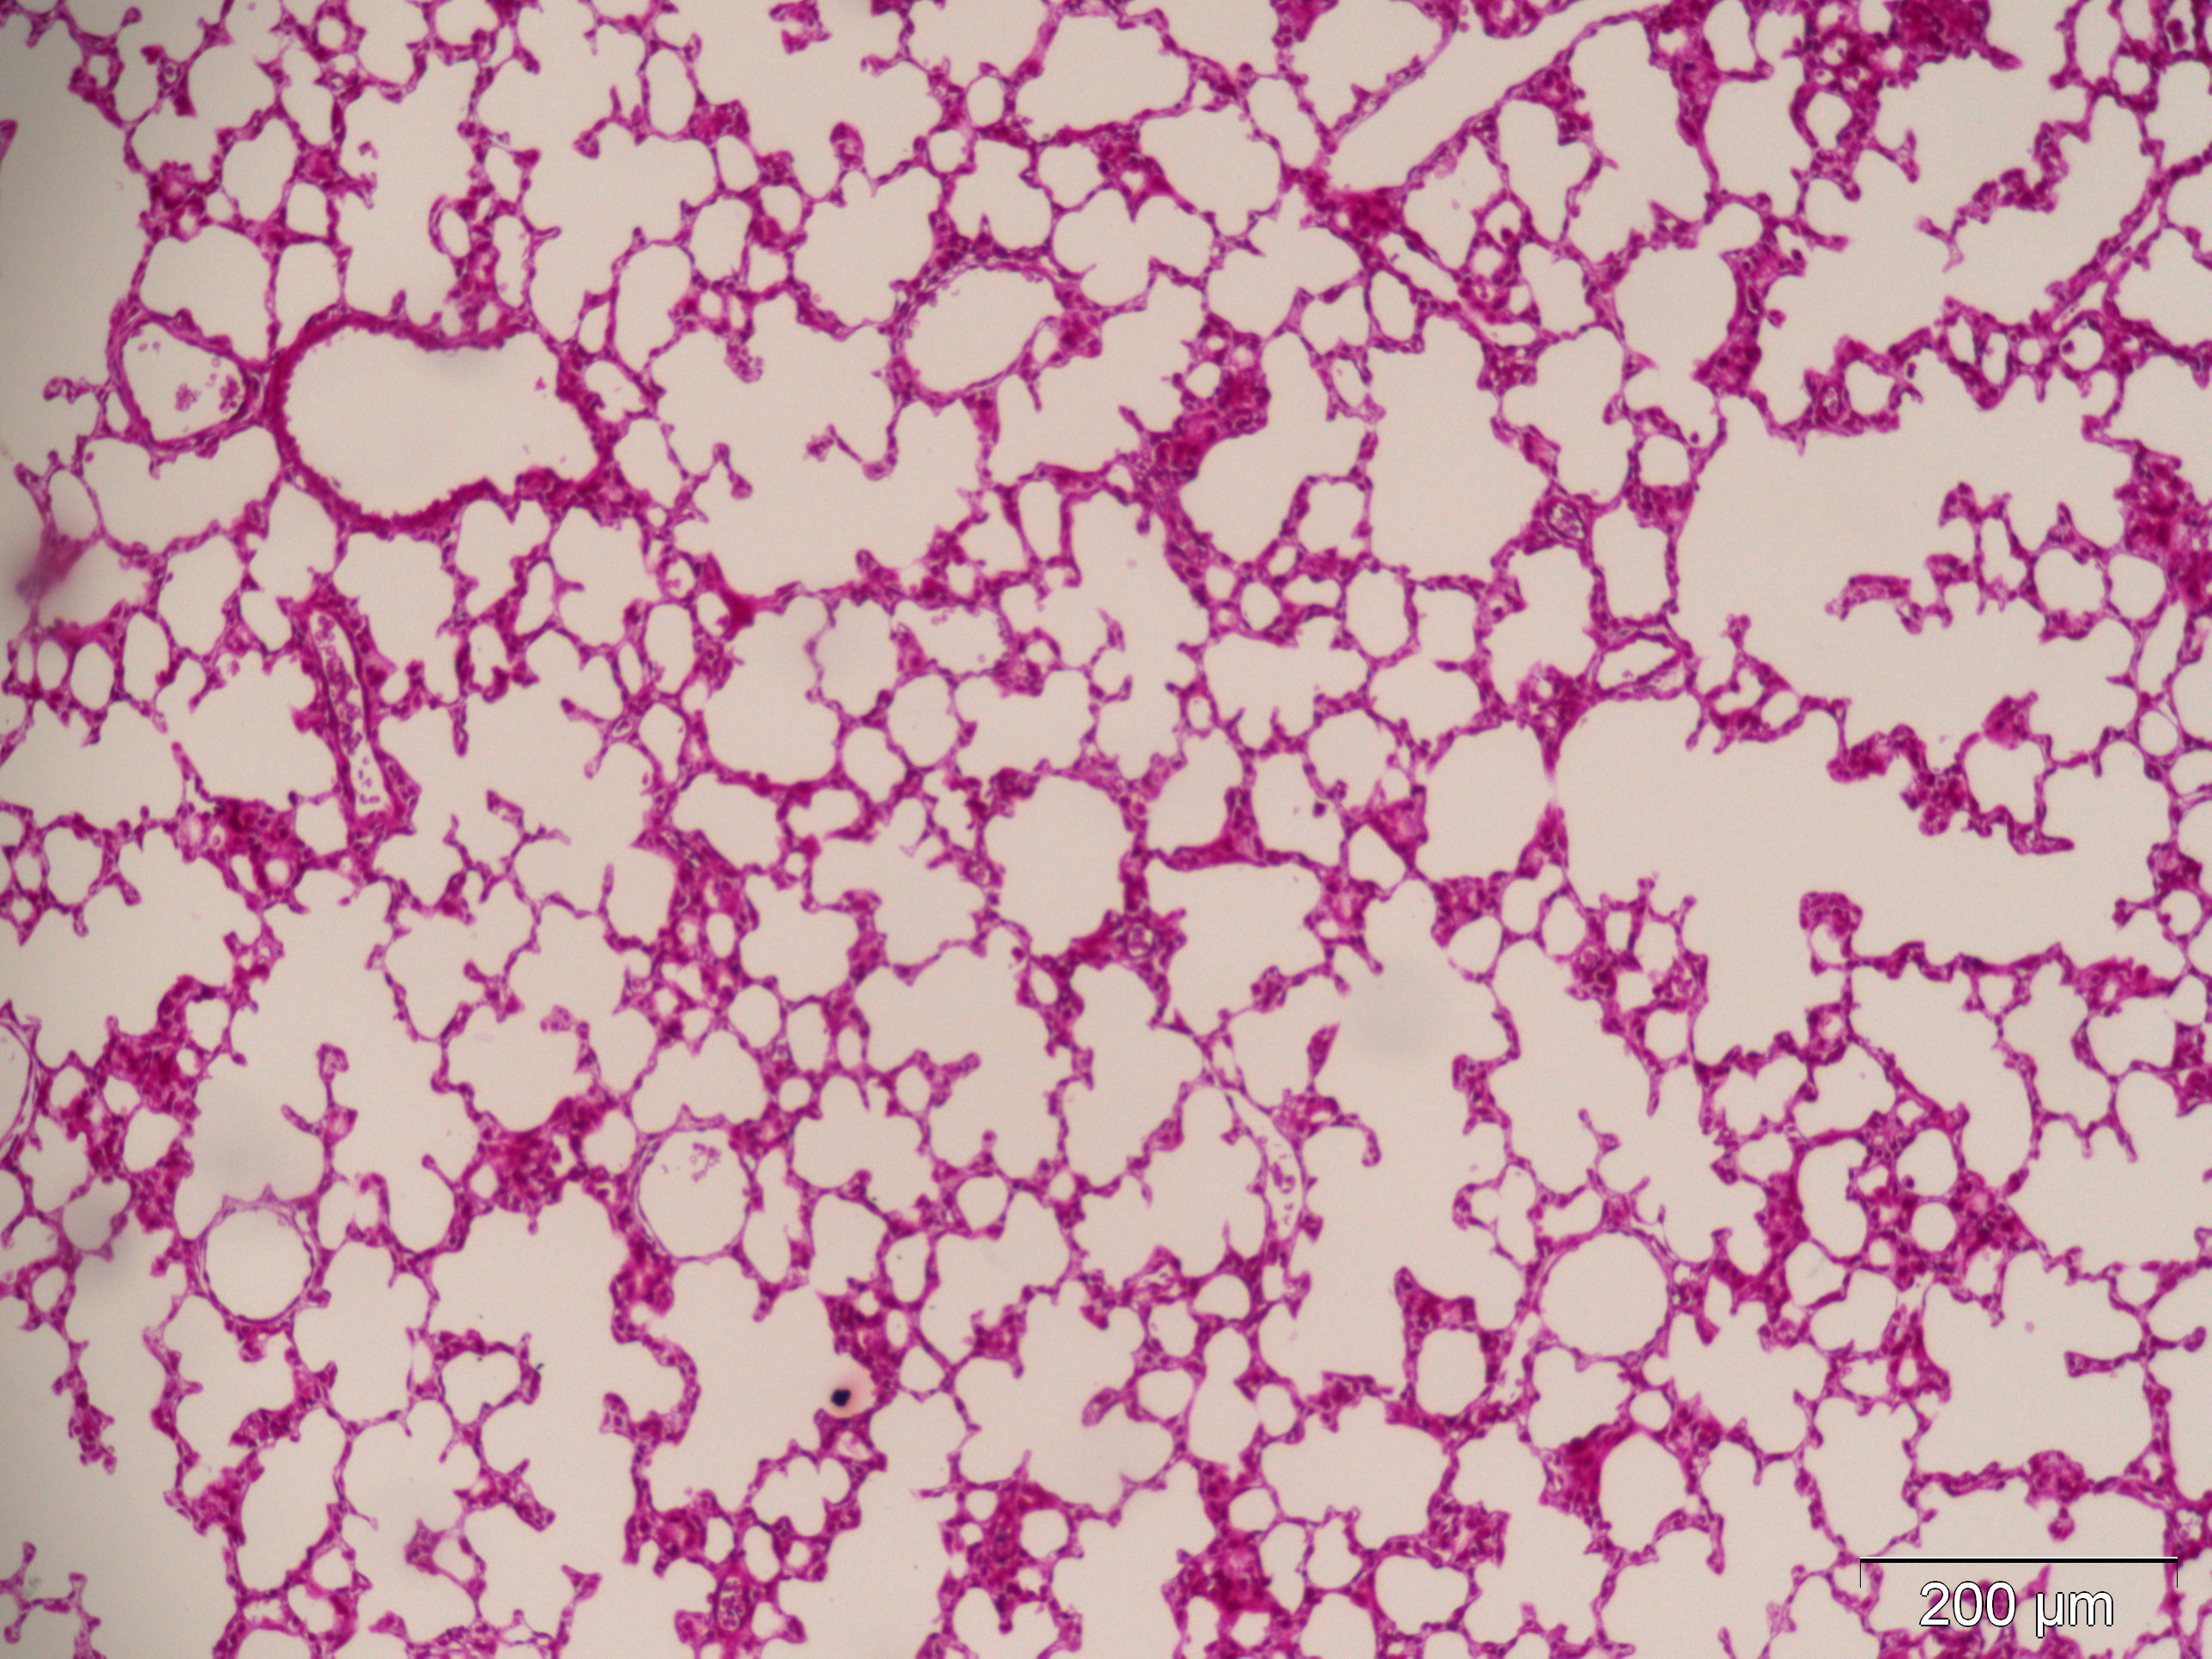
\includegraphics[width=\imsize]{../JPGs/R108C10C_I_8_1_my}
		}
	\subfloat[Full reconstructed slice from the tomographic dataset.]{
		\pgfmathsetlength{\imagewidth}{\imsize}%
		\pgfmathsetlength{\imagescale}{\imagewidth/2936}%
		\def\x{1814}% scalebar-x starting at golden ratio of image width of 2936px = 1814
		\def\y{2642}% scalebar-y at 90% of image height of 2936px = 2642
		\def\mag{4}% magnification of inset
		\def\size{75}% size of inset
		\def\shadow{4}% shadow parameter for scalebar
		\begin{tikzpicture}[x=\imagescale,y=-\imagescale, spy using outlines={rectangle, magnification=\mag, size=\size, connect spies}]
			\begin{scope}
				\clip (0,0) rectangle (2936,2936);
				%\clip (1468.0,1468.0) circle (1468.0);
				\node[anchor=north west, inner sep=0pt, outer sep=0pt] at (0,0) {\includegraphics[width=\imagewidth]{../Originals_TOMCAT/{{R108C10C_B1_mrg1024.rec.8bit}}}};
			\end{scope}
			% \spy [red] on (2636,2636) in node at (0,0) [anchor=north west];
			% 2936px = 4.34528mm > 100px = 148um > 338px = 500um, 68px = 100um
			%\draw[|-|,blue,thick] (0,1468) -- (2936,1468) node [sloped,midway,above,fill=white,semitransparent,text opacity=1] {\SI{4.34528}{\milli\meter} (2936px) TEMPORARY!};
			\draw[|-|,thick] (\x+\shadow,\y+\shadow) -- (\x+338+\shadow,\y+\shadow) node [midway, above] {\SI{500}{\micro\meter}};
			\draw[|-|,white,thick] (\x,\y) -- (\x+338,\y) node [midway,above] {\SI{500}{\micro\meter}};
			%\draw[color=red, anchor=south west] (0,2936) node [fill=white, semitransparent] {Legend} node {Legend};
		\end{tikzpicture}%
	}
	\subfloat[Detail (middle slice) from acinus 32.
		   The segmented acinus is shown in light grey inset into the original data.
		   Scale bar is \SI{100}{\micro\meter}]{
			   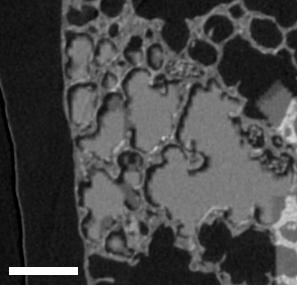
\includegraphics[width=\imsize]{../Originals_TOMCAT/R108C10C_B1_mrg-acinus32_17_a}
		}
%-------------
\end{figure}
\end{document}